\chapter{Monte Carlo Simülasyonu ve Data Üretimi}
\section{Monte Carlo Simülasyonu}
Rastgele üretilen sayılardan daydalanılarak istatistiksel simülasyonlar Monte Carlo (MC)\footnote{Los Alamos Bilimsel Laboratuar’ından John Von Neumann, Stan Ulam ve Nick Metropolis adlarında üç bilim adamı tarafından ortaya çıkarılmıştır. Metropolis algoritması olarak da bilinir.} metoduyla yapılır. 
Deney girdileri belirli olmayan, kesin olmayan bir sekilde gelmesi bekleniyorsa ve dağılım bir fonksiyonla hesaplanabilecekse kullanılır. MC, rastgele sayıları baz alarak tahmini sistemleri modeller. MC methodunun kullanıldığı bazı alanlar, Sayisal Analiz, Atom ve Molekul Fiziği, Nükleer Fizik, Yüksek Enerji Fiziği gibi alanlarda modellerle test edilebilen simulasyonlar gerçekleştirilir. 
\par 1930 yılında İtalyan bir fizikçi olan Enrico Fermi’nin, yeni keşfedilmiş olan nötronun özelliklerinin hesaplaması sırasında Monte Carlo Yöntemi’ni kullanması ile bu yöntemin adı duyulmuş oldu. Sınırlı hesaplama kaynaklarına sahip olunduğunda sıklıkla kullanılan bir yöntemdir. Örnek olarak Monte Carlo Yöntemi İkinci Dünya Savaşı sırasında ilk atom bombasının geliştirildiği Manhattan Projesi’nde kullanılmıştır. MC yönteminde yüksek boyutlu integrallerin çözümünü daha kolaylaştırmakta ve hata oranı işlem yapılmadan önce yaklaşık olarak rahatlıkla kestirilebilmektedir  
\begin{equation}
I= \int_{x_1}^{x_2} f(x) dx \equiv (x_2 - x_1) \frac{1}{N}\sum_{i=1}^N f(x_i)
\end{equation}
\par $x= (x^1,x^2,\cdots ,x^d)$, $d$ integral boyutunu göstermek üzere, integrali toplam şeklinde gösterimi:
\begin{equation}
I=\int_R f(x) dx = \triangle x^d \sum_{i_1 =1}^N \sum_{i_2 =1}^N \cdots \sum_{i_d =1}^N f(x_{i_1}^1,\cdots,x_{i_d}^d)
\end{equation}
şeklinde ifade edebiliriz. Her bir boyut için 10 adet örnek eleman kullandığımızda yapmamız gereken işlem sayısı $N^d =10^5=100000$ dir. MC için hata oranı $\left(\frac{1}{\sqrt{N}}=\frac{1}{\sqrt{100000}}=0.00316 \right)$ dir.
\par \textbf{\textit{MC yöntemine ait bir kaç teknik mevcuttur.}}
\par \textbf{Reddetme yöntemi: \footnote{Rejetion Method} } Sekil \ref{fig:reject} seçilen rastgele noktalar eğer $f(x)$ fonksiyonuna ait eğrinin altında kalıyorsa kabul, değilse reddedilerek toplam yapılan denemelerden kaç tanesinin başarılı sonuç verdiği hesaplanır. Yapılan işlemler sonucunda, toplam deneme sayısının başarılı deneme sayısına oranı, toplam alanın integrali alanın integrali alınarak istenilen $f(x)$ fonksiyonunun alanına oranını verir.
\par Bu yöntem bir veya daha fazla keskin tepe noktası olan fonksiyonlar için uygun bir yontem değildir. Reddedilen noktalar vakit kaybına sebeb olur şekil \ref{fig:reject2}

%%%%%%%%%%%%%%%%%%%%%%%%%%%%%%%%%%%%%%%%%%%%%%%%%%%%
\begin{figure}[!htpb]
        \centering
        \begin{subfigure}[b]{0.35\textwidth}
            \centering
            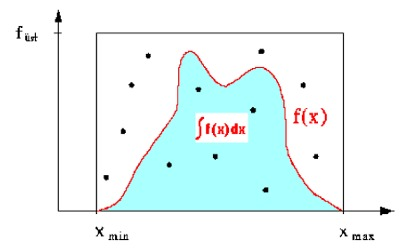
\includegraphics[width=\textwidth]{reject}
            \caption[Reddetme yontemi]%
            {{\small Reddetme yontemi}}    
            \label{fig:reject}
        \end{subfigure}
        \hfill
        \begin{subfigure}[b]{0.35\textwidth}  
            \centering 
            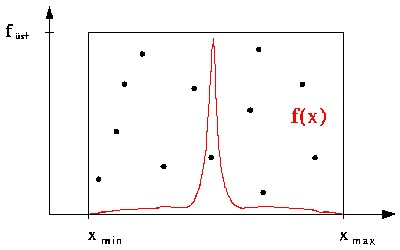
\includegraphics[width=\textwidth]{reject2}
            \caption[keskin tepe noktasina sahi olan fonksiyon]%
            {{\small keskin tepe noktasina sahi olan fonksiyon}}    
            \label{fig:reject2}
        \end{subfigure}
        \vskip\baselineskip
        \begin{subfigure}[b]{0.35\textwidth}   
            \centering 
            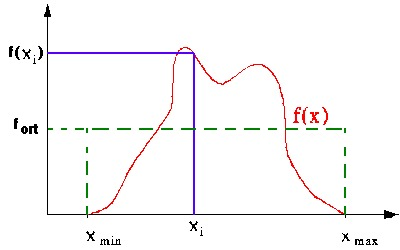
\includegraphics[width=\textwidth]{average_mc}
            \caption[Monte Carlo icin ortalama yontemi]%
            {{\small Monte Carlo icin ortalama yontemi}}    
            \label{fig:avarage}
        \end{subfigure}
        \quad
        \begin{subfigure}[b]{0.35\textwidth}   
            \centering 
            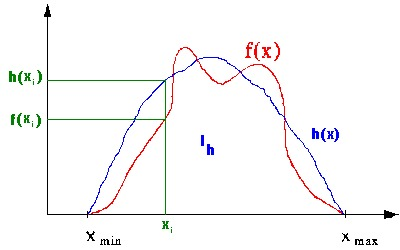
\includegraphics[width=\textwidth]{kontrol}
            \caption[Kontrol Degiskeni Yontemi]%
            {{\small Kontrol Degiskeni Yontemi}}    
            \label{fig:kontrol}
        \end{subfigure}
        \caption[ Monte Carlo Yontemleri]
        {\small Monte Carlo Yontemleri} 
        \label{fig:MonteCarlo}
    \end{figure}

%%%%%%%%%%%%%%%%%%%%%%%%%%%%%%%%%%%%%%%%%%%%%%%%%%%%

\par \textbf{Ortalama Yöntemi : \footnote{Averaging Method}} Şekil \ref{fig:avarage} görüldüğü gibi ortalama yöntemide rastgele seçilen noktalar üzerinden işlem yapar. Reddetme yönteminden farklı olarak, alan taramak yerine, seçilen noktalardaki fonksiyonun değerinden yola çıkarak sonucu bulmaya çalışır.


\par \textbf{Kontrol Değişkeni Yöntemi : \footnote{Control Variates Method}} Bu yöntemde, integrali alınmak istenen $f(x)$ fonksiyonuna oldukça yakın bir $h(x)$ yardımcı fonksiyonu kullanılır. Bu yardımcı fonksiyonun integral değeri, $f(x)$ fonksiyonumuzdan daha kolay hesaplanabilir veya çözümü bilinen bir fonksiyon olmalıdır .Böylelikle seçilen her rastgele noktada iki fonksiyonun farkından, integral değerleri arasındaki fark bulunmaya çalışılır. Elde edilen fark değeri $h(x)$ fonksiyonunun integral değerine eklenerek $f(x)$ fonksiyonuna ulaşılmaya çalışılır. \ref{fig:kontrol}


\begin{equation}
\begin{aligned}
\textbf{ Monte Carlo } \varpropto \frac{1}{\sqrt{N}}\\
\textbf{Trapezium } \varpropto \frac{1}{N^{\frac{2}{d}}}\\
\textbf{Simpson's } \varpropto \frac{1}{N^{\frac{4}{d}}}\\
\end{aligned}
\end{equation}
\par Yukarıda görüldüğü uzere Monte Carlo metodu diğer yöntemlere göre integralin boyutuna bağlı değildir. Bu yüzden MC yönteminde eğer tek katlı integral çözümü yapılacaksa zaman alabilir ancak çok katlı integrallerde MC yöntemi integralin boyutundan bağımsız olduğu için açık ara bir avantaj sağlayacaktır.

\par Matematikte ve fizikte bir faz uzayı içinde bir sistemin tüm olası durumlarının temsil edildiği bir uzaydır. Sistemin her olası durumuna karşılık faz uzayında bir tek nokta vardır. Parçacık çarpışma işleminde teorik olarak çok katlı integrallerin çözümleri gerekmektedir. Eğer son durumda $n$ adet parçacık varsa $d=3 n - 4 $ adet faz uzayı mevcuttur. 2 parçacığın çarpışıp 3,4,...,n parçacıklarını ürettiklerini varsayalım:
\begin{equation}
1+2 \rightarrow 3 + 4 + ... + n
\end{equation}
\par Sacılma tesir kesiti,
\begin{equation}
\begin{aligned}
\sigma=  \frac{S \hbar^2}{4\sqrt{(p_1 \cdot p_2)^2 - (m_1 m_2 c^2)^2}}\int |\mathscr{M}|^2 (2 \pi)^4 \delta^4(p_1 + p_2 - p_3 \cdots - p_n) \\ \times \prod_{j=3}^n \frac{1}{2\sqrt{\textbf{p}_j^2+m_j^2c^2}}\frac{d^3 \textbf{p}_j}{(2\pi)^3} 
 \end{aligned}
\end{equation}
dormülü ile verilir. Burada $p_i$ $i$. parçacığın 4-vektör momentumudur (kütlesi $m_i$) ve $S$ istatistiksel düzeltme faktörüdür. Örnek olarak, $a \rightarrow b + b +c +c +c$ gibi bir sureç için $S= (1/2!)(1/3!)=1/12$ olur. $\mathscr{M}$ ise genliği belirtmektedir\footnote{$\mathscr{M}$ nin nasıl elde edileceği Ekler Kısmında Bir Oyuncak Kuram İçin Feynman kurallarında anlatılmıştır}.

\section{Olay Üretimi}
\subsection{MadGraph}
MadGraph\footnote{MadGraph'in ilk versiyonu Fortran'da 1994 yılımda  Tim Stelzer tarafından yazılmıştır.} programı yüksek enerji fiziğinde parçacık çarpıştırmasında parçacıkların son durumlarını veren ve MC metodunu kullanan bir similasyon yazılımıdır.Ağaç seviyesinde matrix elemanı hesaplayıcısı, tesir kesiti hesabı ve olay üretimi yapan MG uzun süre C++/Fortran ile hazırlanan MG4, 2010 yılından bu yana Python dilinde hazırlanan MG5 i kullanmaktadır. MG5 Grid üzerinde, çok çekirdekli ya da küme bilgisayarlarda başarılı hesaplamalar yapabilmektedir. 
\begin{figure}[!htpb]
\centering
	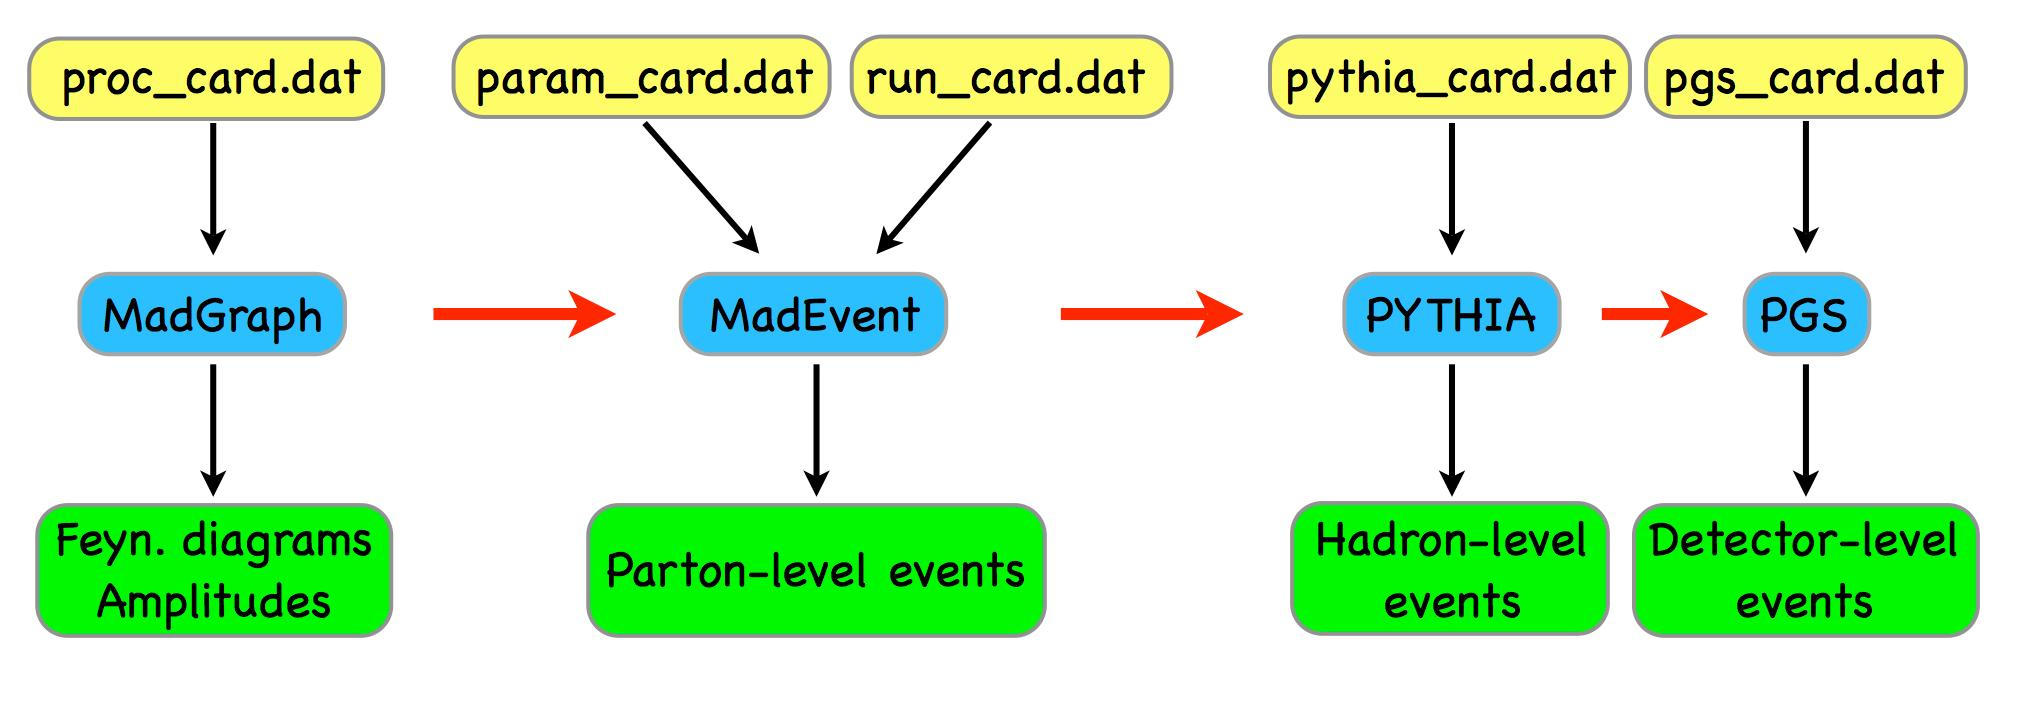
\includegraphics[scale=0.2]{madgraphwork}
	\caption{MadGraph programının çalışma şeması}
	\label{fig:mgwork}
\end{figure}

Şekil \ref{fig:mgterminal} de görüldüğü üzere kullanıcı arayüzü yoktur. Terminal üzerinden çalıştırılır. Sonuçları HTML olarak verir.


\begin{figure}[!htpb]
\centering
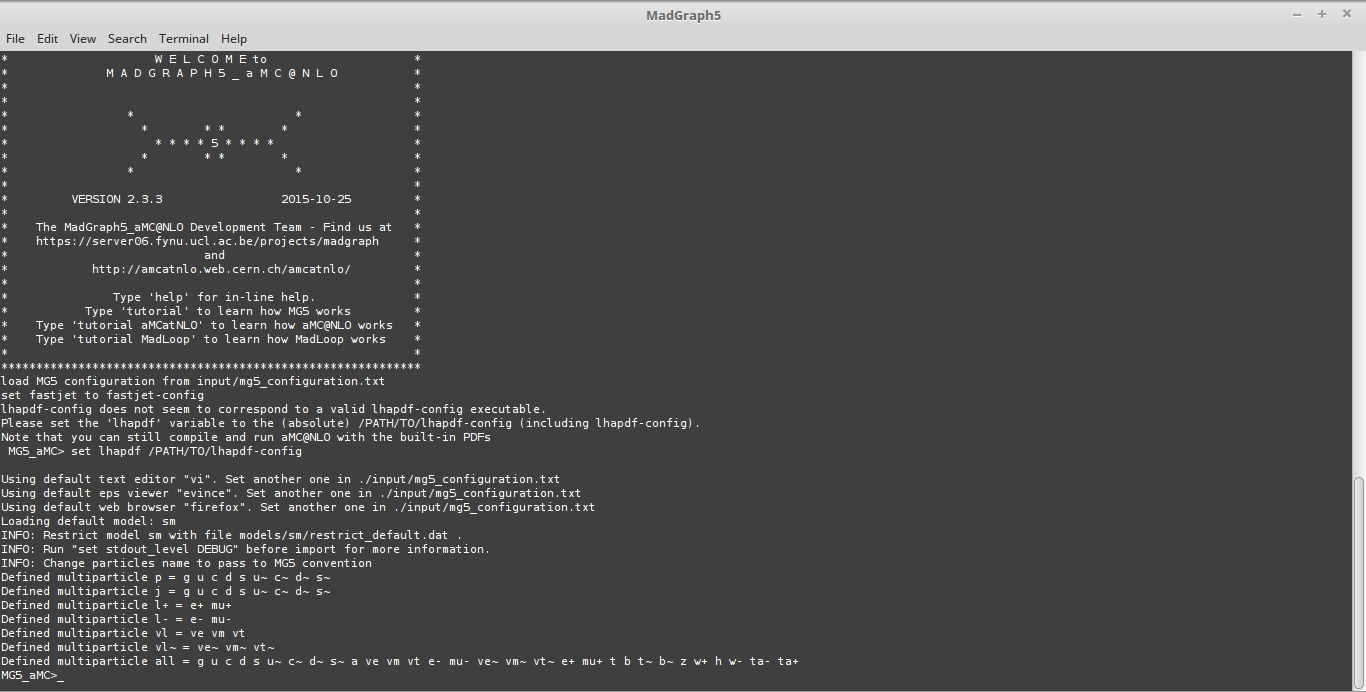
\includegraphics[scale=0.3]{madgraph5}
\caption{MadGraph programının teminal üzerinde görüntüsü}
\label{fig:mgterminal}
\end{figure}


MadGraph programı açık kaynak koddur ve kurulumu bir kaç basit adımda gerçekleştirilebilir\footnote{Ekler kısmında MadGraph kurulumu anlatılmıştır.}. MG çalışma prensibi ve çalışma adımları. 


\par \textbf{MadGraph : } 
\par MadGraph da olay üretimi için $proc\_card.dat$ dosyasını kullanır.

\begin{lstlisting}
import model sm-no_b_mass
define p = g u c d u~ c~ d~ s~
generate p p > j j
output 100-250
\end{lstlisting}
\texttt{ import model }satırında kullanmak istediğimiz modelimizi tanımlıyoruz. Daha sonra parçacıkların ne içerdiğini  \texttt{define} ile belirtiyoruz. \texttt{generate} komutu ile istediğimiz olayı tanımlayıp olay üretimimizi başlatabiliriz. Olay üretimi başladıktan sonra MG ilk olarak istenilen Feynman diyagramlarını çıkartıyor. 

\begin{figure}[!htpb]
\centering
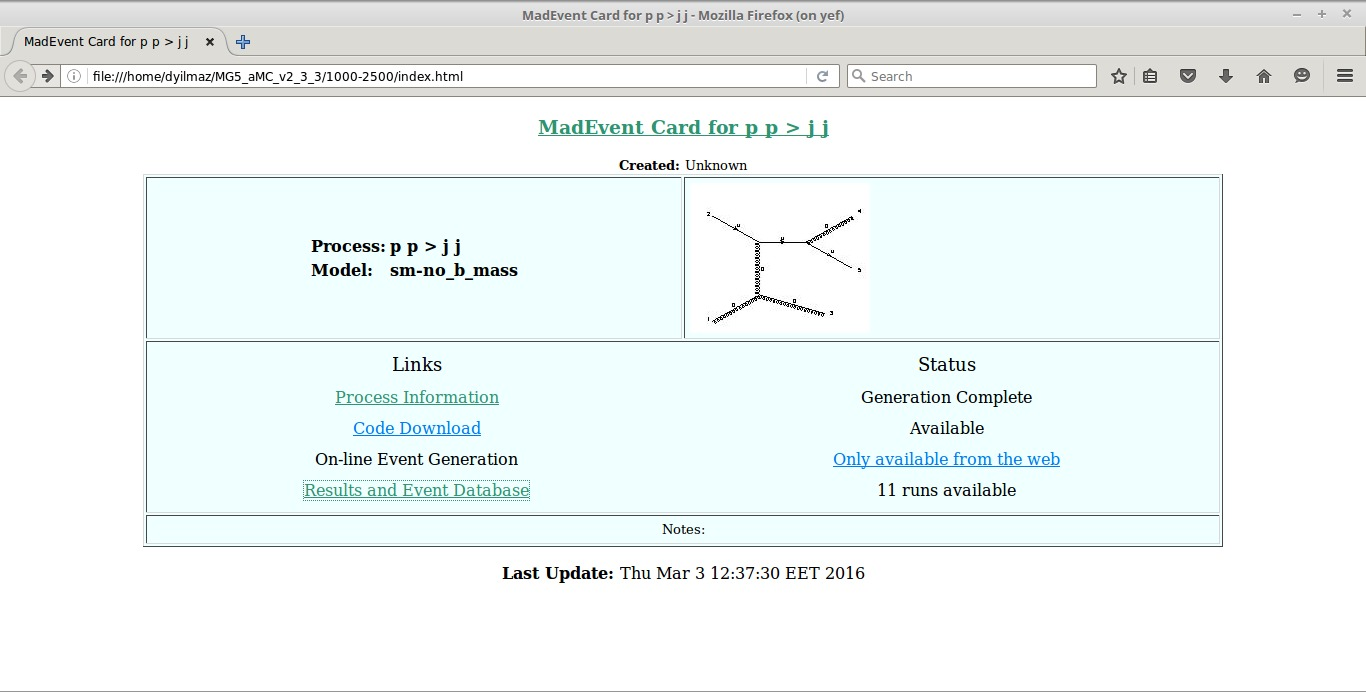
\includegraphics[scale=0.3]{madgraphsecreen}
\caption{MadGraph programının analiz sonucu HTML çıktısı}
\label{fig:mgscreen}
\end{figure}

\par \textbf{MadGraph Feynman Diyagramları Üretimi}\footnote{Anlatılan kartların içeriği Ekler kısmında mevcuttur.}
MG içerisinde $proc\_card.dat$ dosyasında kullandığımız model \texttt{models} adlı klasörde kullandığımız model\footnote{Biz olay üretimimizde sm-no\_b\_mass kullandık} klasöründe; parçacık bilgilerini, köşegen bilgilerini ve diğer bilgileri kullanarak Feynman kurallarına uygun Feynman diyagramlarını çıkartıyor. Birkaç örnek olarak;

Kuplaj parametreleri couplings.py dosyasıyla;
\begin{lstlisting}
GC_1 = Coupling(name = 'GC_1',
                value = '-(ee*complex(0,1))/3.',
                order = {'QED':1})
                
GC_44 = Coupling(name = 'GC_44',
                 value = '(CKM2x1*ee*complex(0,1))/(sw*cmath.sqrt(2))',
                 order = {'QED':1})
\end{lstlisting}
Kuplaj sabitlerini belirliyor. Ayrıca köşegenler için ise vertices.py;
\begin{lstlisting}
V_1 = Vertex(name = 'V_1',
             particles = [ P.G0, P.G0, P.G0, P.G0 ],
             color = [ '1' ],
             lorentz = [ L.SSSS1 ],
             couplings = {(0,0):C.GC_33})
             
V_46 = Vertex(name = 'V_46',
              particles = [ P.a, P.W__plus__, P.G__minus__ ],
              color = [ '1' ],
              lorentz = [ L.VVS1 ],
              couplings = {(0,0):C.GC_75})
\end{lstlisting}
ayrıca decays.py;
\begin{lstlisting}
Decay_e__minus__ = Decay(name = 'Decay_e__minus__',
                         particle = P.e__minus__,
                         partial_widths = {(P.W__minus__,P.ve):'((Me**2 - MW**2)*((ee**2*Me**2)/(2.*sw**2) + (ee**2*Me**4)/(2.*MW**2*sw**2) - (ee**2*MW**2)/sw**2))/(32.*cmath.pi*abs(Me)**3)'})
                         
Decay_ta__minus__ = Decay(name = 'Decay_ta__minus__',
                          particle = P.ta__minus__,
                          partial_widths = {(P.W__minus__,P.vt):'((MTA**2 - MW**2)*((ee**2*MTA**2)/(2.*sw**2) + (ee**2*MTA**4)/(2.*MW**2*sw**2) - (ee**2*MW**2)/sw**2))/(32.*cmath.pi*abs(MTA)**3)'})

\end{lstlisting}
elektron anti tau gibi parçacıkların decay bilgilerini tanımlıyor.\\

\par \textbf{MadEvent} 
\par MadEvent kısmında MG programı $param\_card.dat$ ve $run\_card.dat$ dosyaları kullanılarak çıkmış olan Feynman diyagramlarının genlikleri ($\mathscr{M}$), saçılma tesir kesiti gibi hesaplamalar yapılmaktadır.


\begin{lstlisting}
#*********************************************************************
  100000 = nevents ! Number of unweighted events requested
  0   = iseed   ! rnd seed (0=assigned automatically=default))
#*********************************************************************
# Collider type and energy                                           *
# lpp: 0=No PDF, 1=proton, -1=antiproton, 2=photon from proton,      *
#                                         3=photon from electron     *
#*********************************************************************
     1        = lpp1    ! beam 1 type 
     1        = lpp2    ! beam 2 type
     6500.0     = ebeam1  ! beam 1 total energy in GeV
     6500.0     = ebeam2  ! beam 2 total energy in GeV
#*********************************************************************
\end{lstlisting}
 $run\_card.dat$ dosyasından kaç tane olay üreteceğimiz, çarpıştıracağımız parçacıkların neler ve hangi enerjide olduklarını ayarlayabiliyoruz.
\begin{lstlisting}
#*********************************************************************
# Minimum and maximum pt's (for max, -1 means no cut)                *
#*********************************************************************
20.0  = ptj       ! minimum pt for the jets 
-1.0  = ptjmax    ! maximum pt for the jets
0.0 = drjj    ! min distance between jets 
-1.0  = drjjmax ! max distance between jets
30.0   = xqcut   ! minimum kt jet measure between partons
\end{lstlisting}
Arıca çıkacak olan Jet lerin minimum enerjisi maksimum enerjisi aralarındaki minimum ve maximum uzaklık gibi son durumda elde etmek istediğimiz parçıkların veya Jetlerin özelliklerini belirleyebiliyoruz. Bu ayarlamaları yaptıktan sonra MadEvent kısmında saçılma tesir kesiti ve genlik hesabı yapılmaktadır ve yapılan bu hesaplamalara göre istediğimiz son durumlar MC yöntemi kullanılara simüle edilmektedir.
\par Hadron çarpıştırıcısında bir tesir kesiti hesabı ;
\begin{equation}
\sigma =\frac{1}{F} \sum_ab  \int dPS^{(n)} dx_a dx_b f_{(a/p)}(x_a) f_{(b/p)}(x_b) \overline{|M_{fi}|^2}
\end{equation}
tüm partonlar üzerinden toplam alınır. Burada $f$ parton dağılım fonksiyonudur (PDF). a ve b protondan gelen birer parton ve x parton fraksiyonları olmak üzere $f(x)$ partonların protonlardan gelme olasılığını gösterir.

\begin{figure}[!h]
\centering
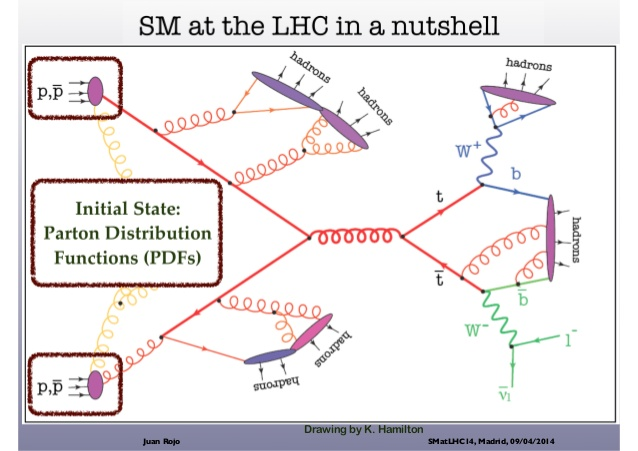
\includegraphics[scale=0.5]{pdf}
\caption{Parton dağılım fonksiyonu ve diğer adımlar}
\label{fig:pdf}
\end{figure}

 Hangi PDF setini kullanacağımızı bu kart içerisinde girebiliriz. Bizim olay üretiminde kullandığımız PDF seti nn23lo1.

\begin{figure}[!htpb]
\centering
\begin{subfigure}[b]{0.5\textwidth}
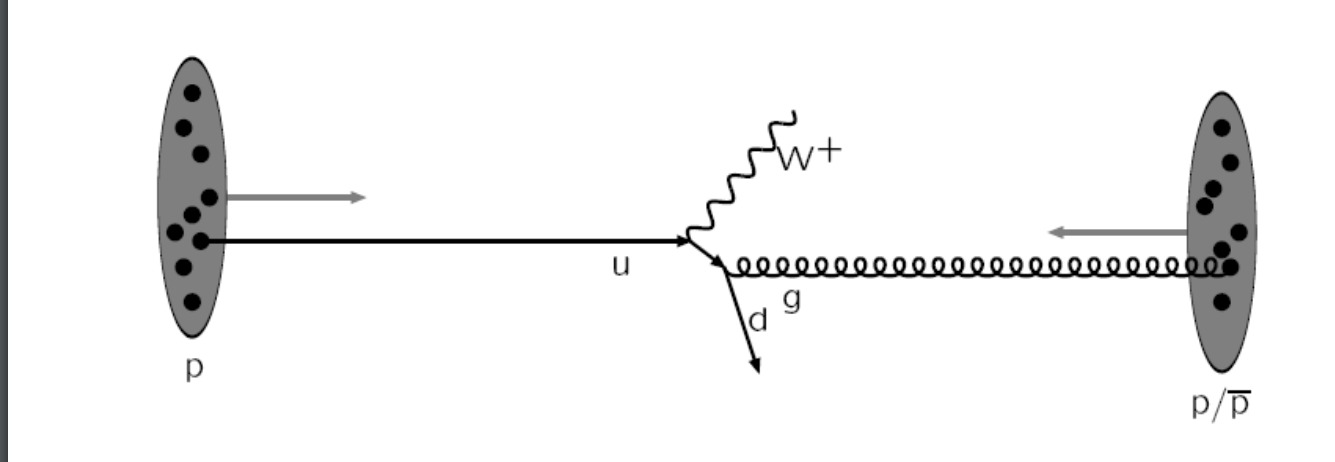
\includegraphics[scale=0.2]{1}
\caption{Sert Saçılma}
\end{subfigure}

\begin{subfigure}[b]{0.5\textwidth}
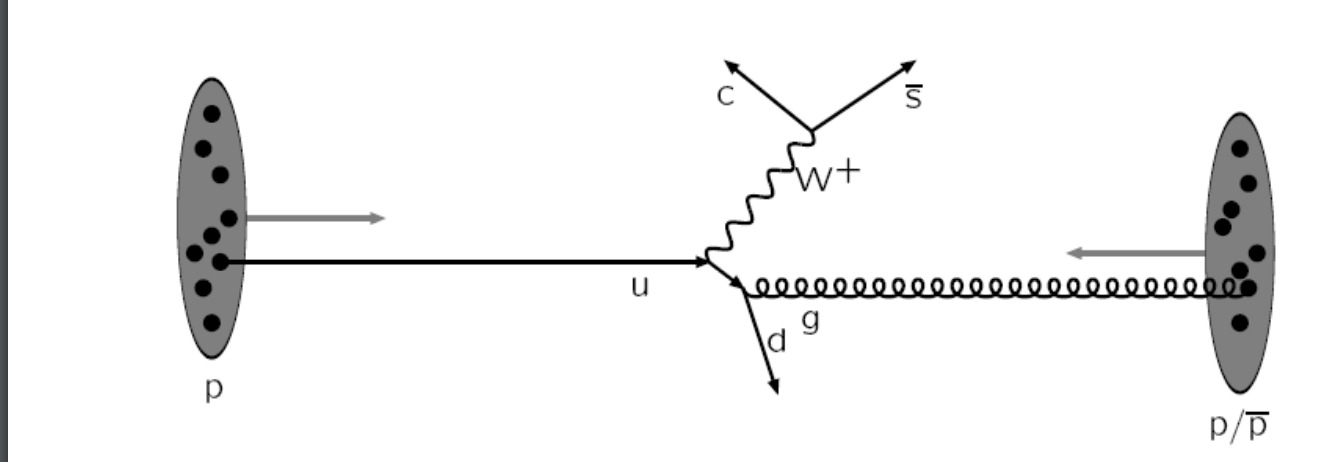
\includegraphics[scale=0.2]{2}
\caption{Alt olay}
\end{subfigure}

\begin{subfigure}[b]{0.5\textwidth}
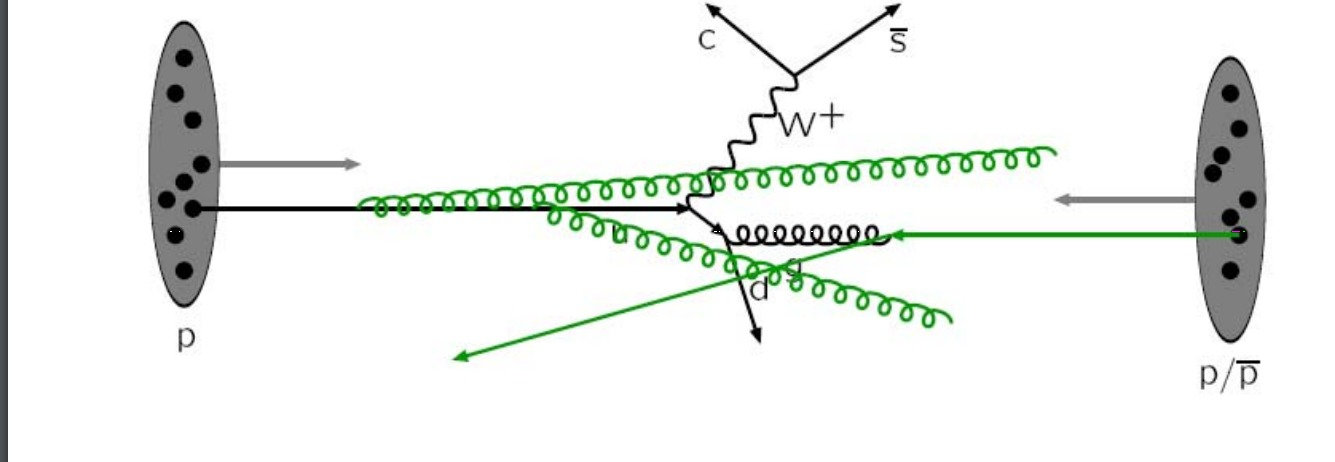
\includegraphics[scale=0.2]{3}
\caption{Başlangıç Durumu Radyasyonu}
\end{subfigure}

\begin{subfigure}[b]{0.5\textwidth}
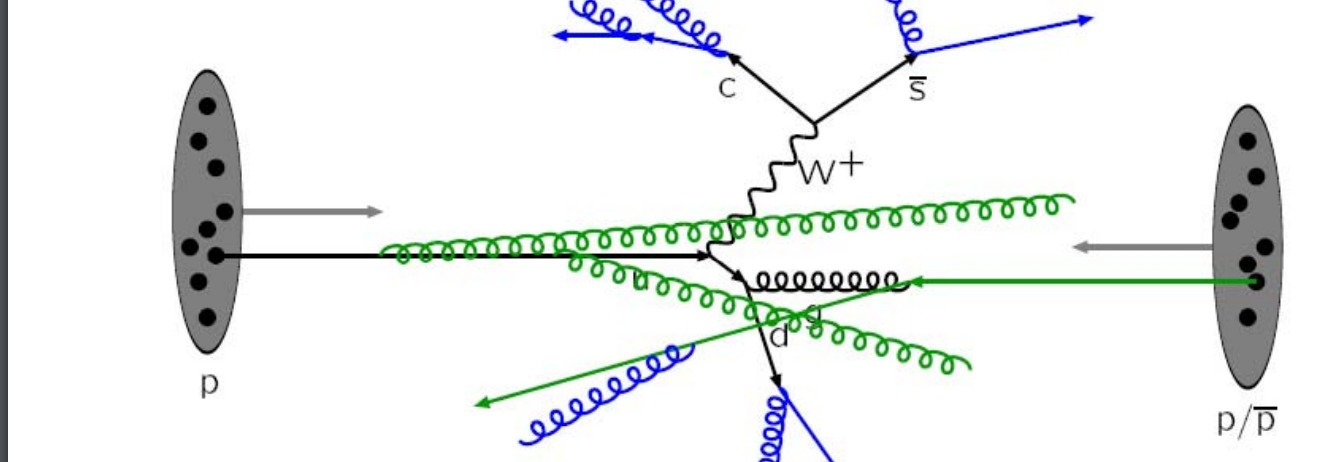
\includegraphics[scale=0.2]{4}
\caption{Son Durum Radyasyonu}
\end{subfigure}

\begin{subfigure}[b]{0.5\textwidth}
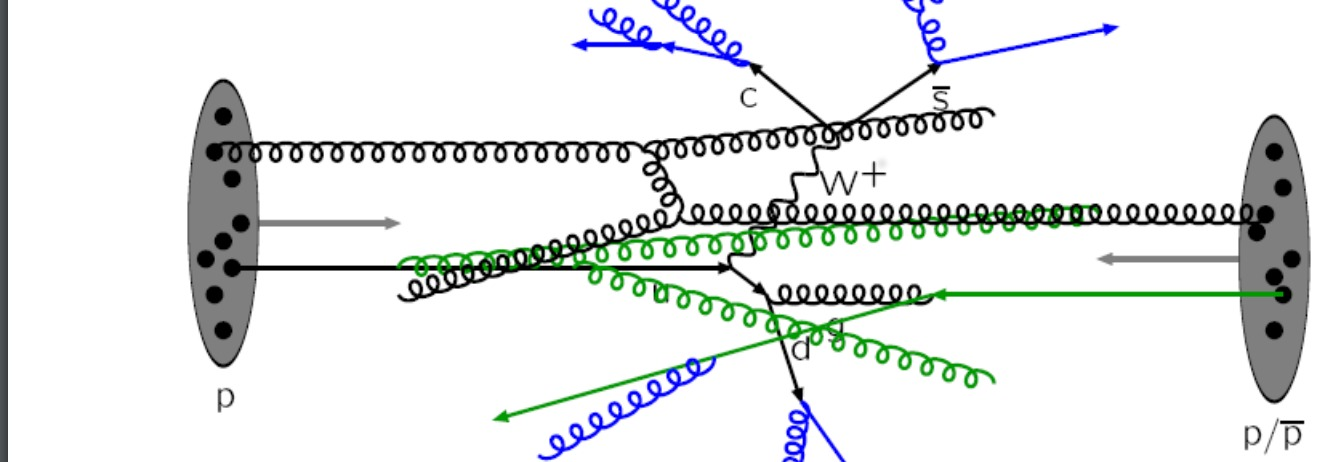
\includegraphics[scale=0.2]{5}
\caption{Çoklu Parton Etkileşimi}
\end{subfigure}
\caption{Proton - Proton Çarpışması adımları}
\end{figure}


\begin{figure}[!h]
		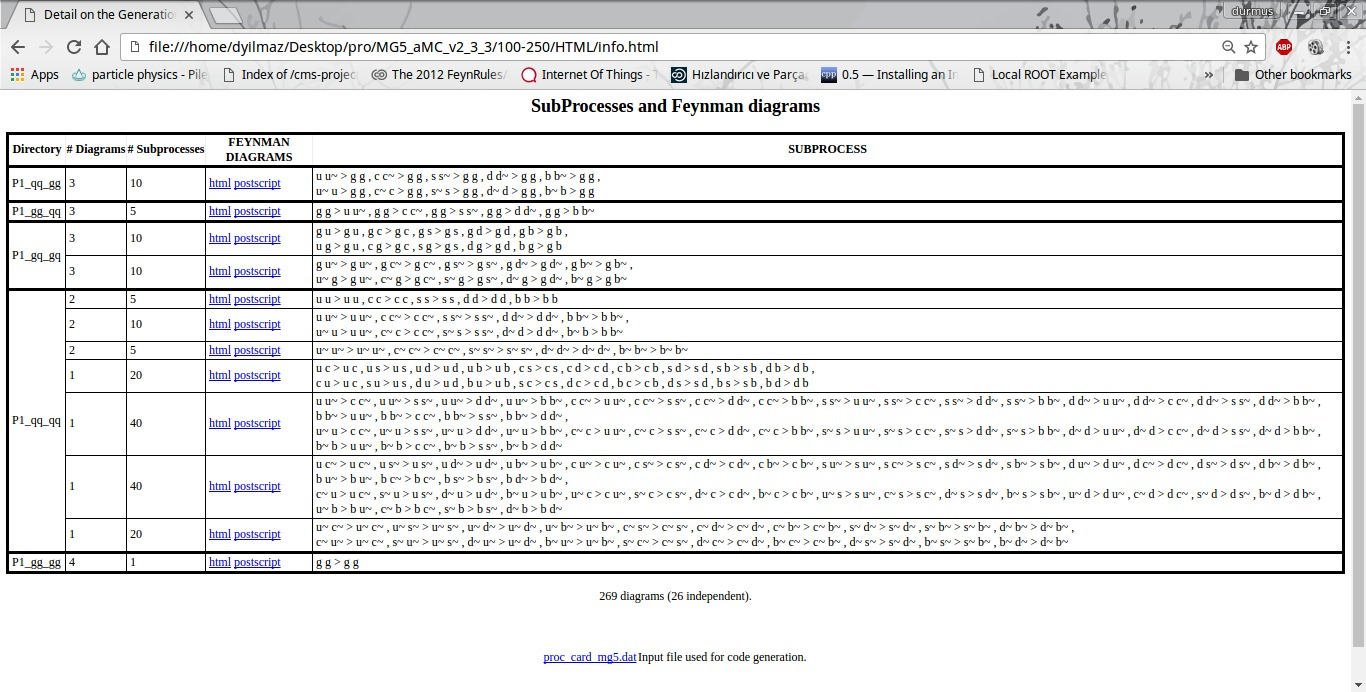
\includegraphics[scale=0.3]{feynrules}
		\caption[p p $>$ j j olayında SM e gore çıkarılan feynman diyagramları]%
        {{\small p p $>$ j j olayında SM e gore çıkarılan feynman diyagramları}}    
        \label{fig:feynrules}
\end{figure}
\par Yüksek Enerji Fiziğinde similasyon için PDG\footnote{PARTICLE NUMBERING SCHEME}(parçacık numaralandırma şeması) 'nın önemli bir yeri vardir. 
Tablo \ref{tab:pdg} bazı önemli parçacıkların PDG leri mevcuttur.\footnote{http://pdg.lbl.gov/2007/reviews/montecarlorpp.pdf}\\
\begin{table}[!htbp]

\centering

\begin{tabular}{|c|c|}

\hline 
\multicolumn{2}{|c|}{Kuarklar} \\ 
\hline 
$d$ & 1 \\ 
\hline 
$u$ & 2 \\ 
\hline 
$s$ & 3 \\ 
\hline 
$c$ & 4 \\ 
\hline 
$b$ & 5 \\ 
\hline 
$t$ & 6 \\ 
\hline 
$b^`$ & 7 \\ 
\hline 
$t^`$ & 8 \\ 
\hline 

\end{tabular} 
\begin{tabular}{|c|c|}

\hline 
\multicolumn{2}{|c|}{Leptonlar} \\ 
\hline 
&\\
\hline 
$e^-$ & 11 \\
\hline 
$\nu_e$ & 12 \\
\hline 
$\mu ^-$ & 13 \\
\hline 
$\nu_\mu$ & 14 \\
\hline 
$\tau^-$ & 15 \\
\hline 
$\nu^\tau$ & 16 \\ 
\hline 

&\\

\hline
\end{tabular}
\begin{tabular}{|c|c|}
\hline 
\multicolumn{2}{|c|}{Bozonlar} \\ 
\hline 
&\\
\hline 
g & 21 \\ 
\hline 
$\gamma$ & 22 \\ 
\hline 
Z & 23 \\ 
\hline 
W & 24 \\ 
\hline 
$h^0 / H^0 $ & 25 \\ 
\hline 
$H^+$ & 37 \\
\hline 
&\\ 
\hline 
\end{tabular} 
\caption{Standart Model deki parçacıkları için PDG kodları}
\label{tab:pdg}
\end{table}


\begin{figure}
\centering
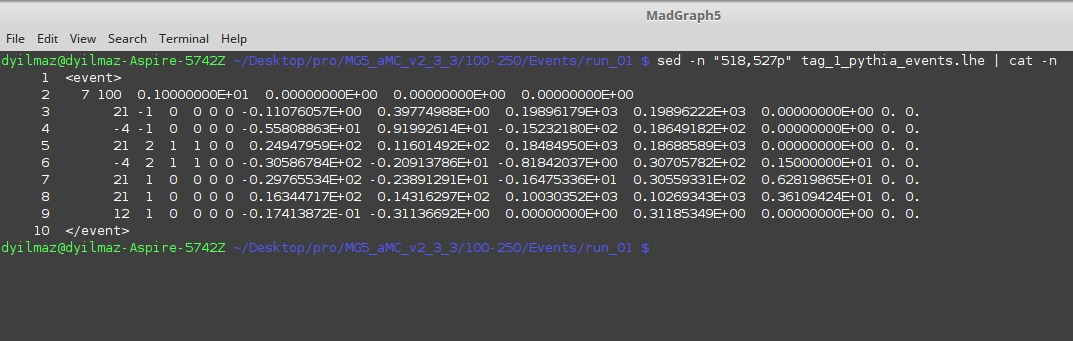
\includegraphics[scale=0.3]{madevent}
\caption{MadEvent çıktı dosyası. İlk satırda çıkan parçacıkların PDG kodları 2. satır başlangıç (-1) son (1) araparçacık (2) bilgisini verir. Ayrıca dört-momuntum ve spin bilgilerinde bu dosyanın içinde mevcuttur.}
\end{figure}

\par \textbf{Pythia}
\par Bu adımda sert saçılma sonrasında parton-duşu\footnote{Parton-Shower} ve hadronizayson yapılmaktadır.Olay üretimimiz sırasında $pythia\_card.dat$ dosyasını kullanmaktadır. Ptyhia gerekli işlemleri yaptıktan sonra bize .HEP\footnote{High Energy Physics} uzantılı dosyayı verir. Artik dedektor similasyonuna sokmadan once elimizde istediğimiz olaya ait verileri almış oluyoruz. \\
Eklerde bulunan $pythia\_card.dat$ dosyasında parton duşunu, hadronisazyonu, çoklu etkileşimi ve kullanacağımız PDF setini seçebiliyoruz. Örnek olarak bizim kullandığımız PDF seti; \\
 \texttt{
	!...PDFset if MG set not supported by pythia-pgs package (set in lhapdf5 or higher)
   \\ LHAID= 10041
      }
\par \textbf{Delphes Similasyonu}
\par Delphes similasyonu ürettiğimiz olaylar üzerinden tıpkı bir dedektör similasyonuna sokulmuş gibi bize dedektör çıktılarını vermektedir. Dedektör similasyonunda ürettiğimiz olayları algıçlar ile etkileşmesi sonucu bizim elimize similasyon verilerini root olarak alırız. Delphes similasyonu $delphes\_card\_CMS.tcl$ kartını kullanmaktadır.
\begin{lstlisting}
 # magnetic field
  set Bz 3.8
\end{lstlisting}
kod satırı ile silindirdeki manyetik alanı ayarlayabiliyoruz.
\begin{lstlisting}
 # algorithm: 1 CDFJetClu, 2 MidPoint, 3 SIScone, 4 kt, 5 Cambridge/Aachen, 6 antikt
  set JetAlgorithm 6
  set ParameterR 0.5

  set JetPTMin 20.0
\end{lstlisting}
ile Jet algoritmalarımızı jet lerin yarıçapları ve minimum jet enerjisini ayarlayarak, similasyonumuzu yönledirebiliyoruz.
\begin{figure}[!h]
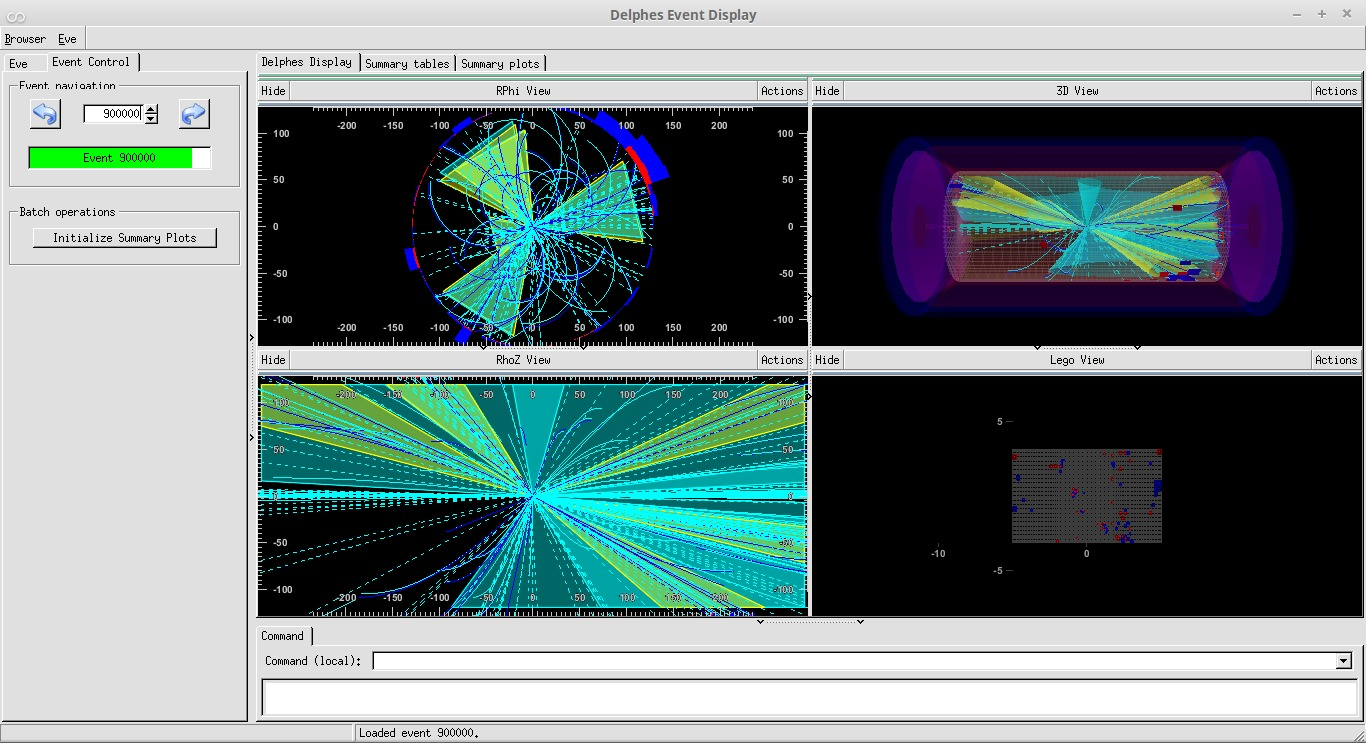
\includegraphics[scale=0.2]{showevent}
\centering
\caption{Delphes Similasyonundan çıkan bir olayın görüntülenmesi}
\label{fig:showevent}
\end{figure}
Şekil \ref{fig:showevent} da göründüğü gibi üretilen bir olayda jetler sınıflandırılmış parçacıklar tanımlanmış ve dedektörün üzerinde hangi parçacığın hangi konumda olduğu hesaplanarak tıpkı gerçek bir olay gibi simüle edilmiş.
\par Deneysel olarak Proton çarpışmasında dedektör üzerine düşen izle hard-disc lere kaylanıyor. Daha sonra bu veriler yeniden yapılandırılarak her bir izin fiziksel karşılığı bulunuyor. Analiz kısmında elde etmiş olduğumuz verilerin histogramları çıkartılıyor. Similasyon kısmında ise MC yöntemş ile yukarıda bahsedilen programlar yardımıyla olaylar simüle ediliyor. Pythia ile dedektör simülasyonundan sonra dedektör üzerindeki izler yeniden yapılandırılıp fiziksel karşılıkları bulunuyor. Analiz kısmında ROOT veya başka bir program ile histogramlar elde ediliyor. Similasyon kısmında teorideki bir model e göre çıkan histogramlar ile deney verisinden eldi edilen veriler karşılaştırılıyor. Eğer deney verisi ile similasyonda farklı sonuçlar verirse teorinin eksik kısımları vardır demek ve düzeltme yapıp tekrardan simülasyon ile deney verileri karşılaştırılıyor. Buna en güzel örnek Standart Model deki Higgs parçacığıdır. Similasyon dan elde edilen veriler ile deneysel veriler karşılaştırıldığında böyle bir parçacığın varlığını ve bu parçacığın özelliklerini tespit edebiliyoruz.



\section{Jet'lerin Yeniden Yapılandırılması ve Algoritmalar}
Kuarklar ve gluon lar renk yüküne sahiptirler({\color{red} r},{\color{green} g},{\color{blue} b}). Kuantum renk dinamiğinin getirdiği kurallardan biri serbest haldeki bir parçacığın renk yükü nötr olmalıdır. Bu yüzden proton-proton çarpışmasında aslında gluon ve kuarkların etkileşmesi incelenirken, serbest halde bulunamayacak olan gluonlar QCD nin izin verdiği müddetçe hadronize olarak kuark antikuark çiftlerine bozulurlar. Böylece bütün renk yükü barındıran parçacıklar hadronizasyon sonucu renksiz parçacıklar oluştururlar.
Jet'ler yüksek enerjili çarpışmalarda açığa çıkan parçacık püskürtüleridir.Kuark ve gluonların dedektörün kalorimetrelerde bıraktıkları enerjilerle tespit edebiliriz. Kısaca parçacık gruplarının oluşturduğu yapıya Jet diyebiliriz. Daha sade bir dil ile söyleyecek olursak jetler yüksek enerji fiziğinde aynı yönde saçılan hadronları tek bir hizaya getirilmiş halleridir. CMS'in yayınladığı araştırmaların $60$ ında Jetler kullanılmıştır. Jetlerin en temel amacı son durumda oluşan karmaşıklığı en aza indirerek basit objeler halinde analiz yapmaktır. Jet algoritmaları için 3 krite vardır. Bunlar collinear güvenilirlik , infrared güvenilirlik ve hız.
\begin{figure}[!htbp]
\centering
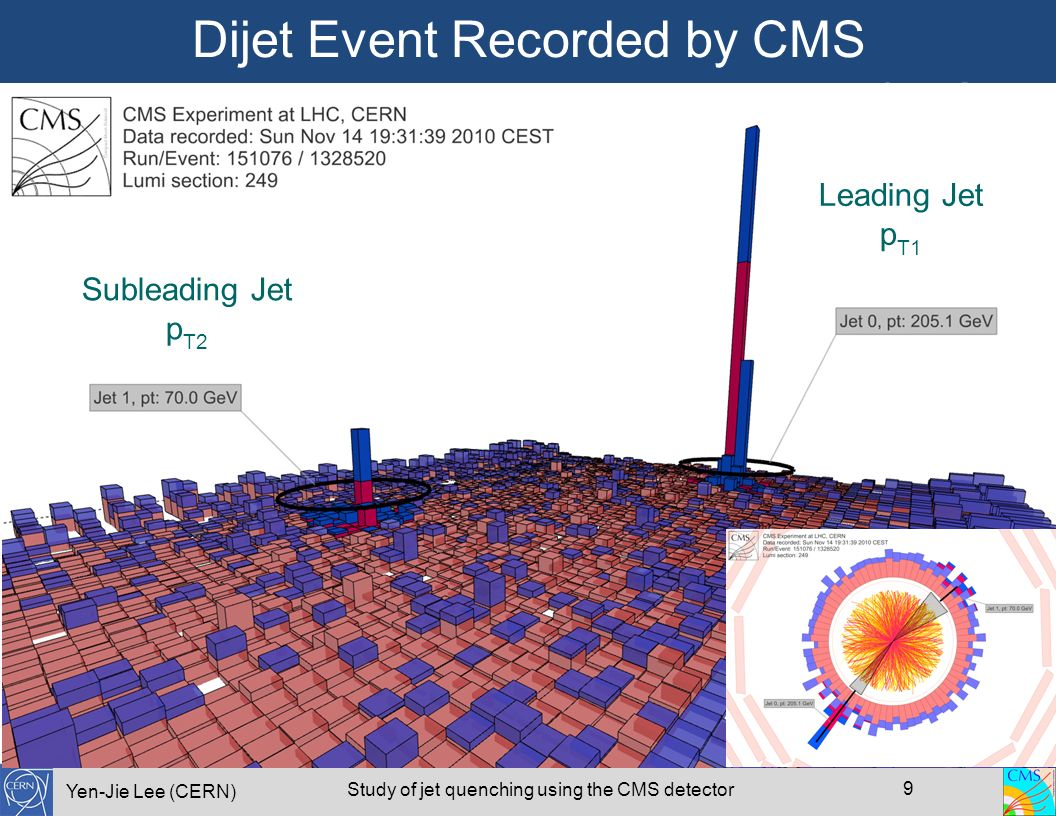
\includegraphics[scale=0.5]{jet}
\caption{2 jet çıkan bir olayın CMS dedektörü üzerindeki izleri}
\label{fig:jet}
\end{figure}

\begin{figure}[!htbp]
\centering


\par Şekil \ref{fig:jet1} de gösterildiği gibi belirlenen bir jet için Jet'in parametreleri;
\begin{equation}
\begin{aligned}
E_{T_{jet}} = \sum_{i \in jet } E_{T_{jet}} \\
\eta_{jet} =\frac{1}{E_{T_{jet}}} \sum_{i \in jet }E_{T_{jet}} \eta_i \\
\phi_{jet} = \frac{1}{E_{T_{jet}}} \sum_{i \in jet }E_{T_{jet}} \phi_i
\end{aligned}
\end{equation}
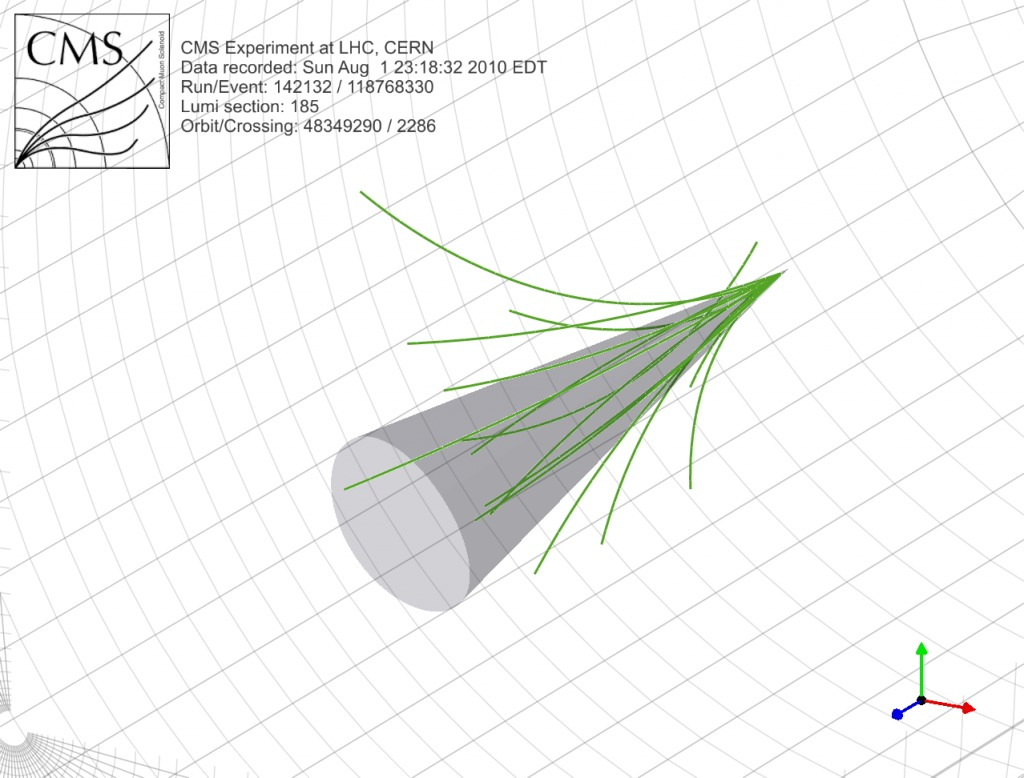
\includegraphics[scale=0.3]{jet1}
\caption{Koni algoritması ile gösterilmiş bir Jet}
\label{fig:jet1}
\end{figure}
\subsection{Jet Algoritmaları}
Temelde iki tip jet algoritma türü vardır. Bunlardan biri koni diğeri kümeleme algoritmasıdır.
\par Koni tipi algoritması kendi içinde 3 e ayrılır. bunlar tekrarlayan koni\footnote{Iterative Cone}  algoritması,  orta nokta \footnote{Midpoint Cone} koni algoritması ve SIS-Cone \footnote{Seedless Infrared-Safe Cone Algorithm}dur. 

\par \textbf{Tekrarlayan koni algoritması} çıkan bütün parçacıkların $p_T$ lerini listeler. Rastgele bir parçacık seçtildikten sonra seçtiğin parçacığın R yarıçaplı bir daire çizerek bu dairenin içinde kalan parçacıkların momentumuna göre tekrar daire çizerek toplar. R yarıçaplı bir dairenin içindeki bütün parçacıkların momentumlarına göre yeniden R yarıçapı çizilerek jet belirlenir.
\begin{figure}[!htbp]
\centering
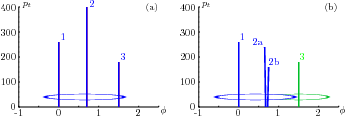
\includegraphics[scale=1]{iterative.png}
\caption{Tekrarlayan koni algoritması en yüksek enerjiye sahip parçacığı seçerek R yarıçapı çemerin içinde kalan bütün parçacıkları toplar}
\end{figure}

\par \textbf{Orta nokta algoritması}Bu algoritmada rastgele ilk jetler belirlenir. Daha sonra her biri için R yarıçaplı daierel çizilir. Eğer iki ilk-jet üst üste geldiyse ve birinin enerjisi diğerinin enerjisinde $\%50$ daha az ise bu bir Jet olarak alınır. 


\par \textbf{SISCONE} 

\par Oldukça hızlı olan bu algoritma CMS tetiklemede kullanılmaktadır. Ancak collinear ve infrared güvenilir değildir.\footnote{collinear ve infrared güvenilirlik Ekler bölümünde anlatılmıştır.}

\par \textbf{Kümeleme Algoritması}\\
Bütün objeler için beam line a olan uzaklık hesaplanır. 
\begin{equation}
d_i = (E_{T,i})^2 \centerdot D^2
\end{equation}

daha sonra diğer parçacıklarla aralarındaki uzaklık hesaplanır.
\begin{equation}
d_{i,j} = min(p_{Ti}^{2p},p_{T j}^{2 p})\frac{\bigtriangleup R_{ij}^2}{R^2}
\end{equation}

\begin{equation}
\bigtriangleup R_{ij}= \sqrt{(y_i-y_j)^2 + (\phi_i - \phi_j)^2} < R
\end{equation}

\par $p=1$ $k_T$ , $p=0$ $Cambridge-Aachen$, $p=-1$ $anti-k_T$ algoritmalarını verir.Tüm parçacıkların birbirinden ve beam-line ndan uzaklıkları belirlenir. Eğer $d_{ij}$ en küçük ise, i ve j parçacıkları birleştirilir ve başa dönülür. Eğer $d_{ib}$ en küçük ise , son durumda Jet olarak belirlenir. Bu işlem hiç bir parçacık kalmayıncaya kadar devam eder.\\
\begin{table}[!htbp]
\centering

\begin{tabular}{|c|c|c|}

\hline 
$k_T$ & $d_{i,j} = min(p_{Ti}^{2p},p_{T j}^{2 p})\frac{\bigtriangleup R_{ij}^2}{R^2}$ & Catani et al ‘91
Ellis, Soper ‘93 \\ 
\hline 
$Cambridge/
Aachen$ & $\frac{\bigtriangleup R_{ij}^2}{R^2}$ & Dokshitzer et al ‘97
Wengler, Wobish ‘98 \\ 
\hline 
$anti-k_T$ & $d_{i,j} = min(p_{Ti}^{2p},p_{T j}^{2 p})\frac{\bigtriangleup R_{ij}^2}{R^2}$ & MC, Salam, Soyez ’08 \\ 
\hline 

\end{tabular} 
\caption{Koni algoritmaları; 2 parçacığın arasındaki mesafe hesabı ve kimin tarafından hangi tarihte yazıldığı}
\end{table}


\begin{figure}
        \centering
        \begin{subfigure}[b]{0.475\textwidth}
            \centering
            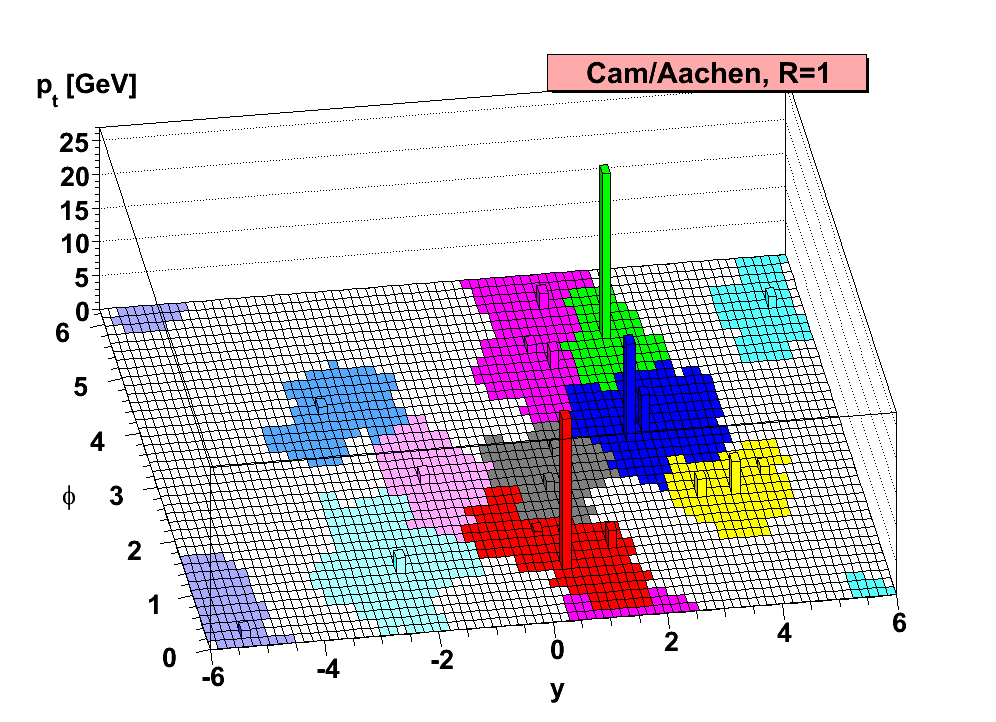
\includegraphics[width=\textwidth]{cam.png}
            \caption[$Cambridge/Aachen$]%
            {{\small $Cambridge/Aachen$}}    
            \label{fig:mean and std of net14}
        \end{subfigure}
        \hfill
        \begin{subfigure}[b]{0.475\textwidth}  
            \centering 
            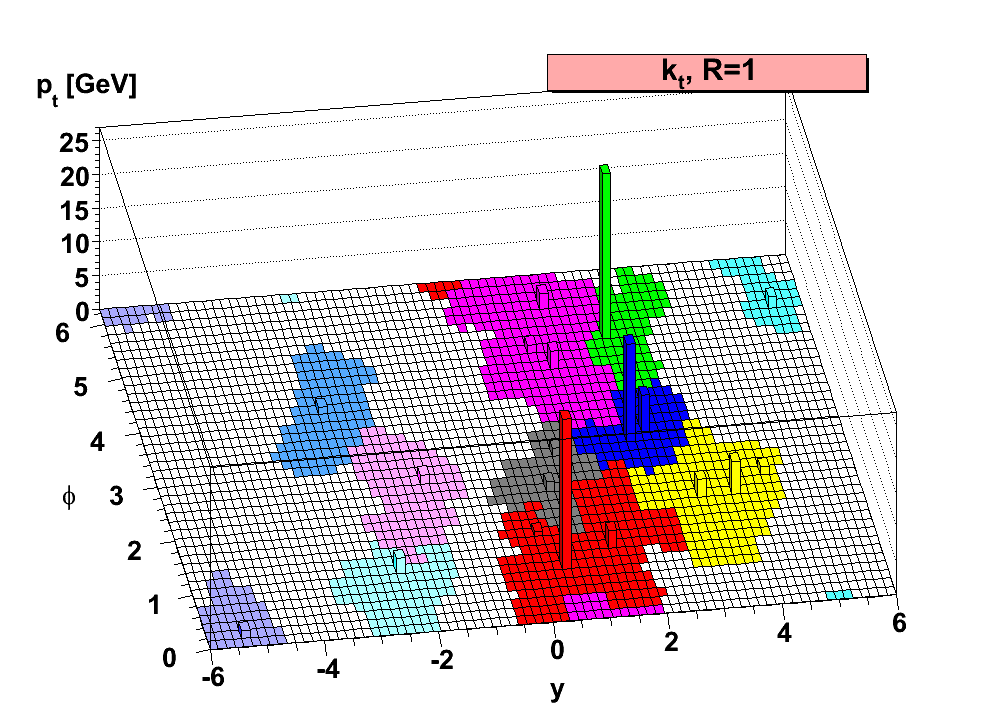
\includegraphics[width=\textwidth]{kt.png}
            \caption[$k_T$ algoritması]%
            {{\small $k_T$ algoritması}}    
            \label{fig:mean and std of net24}
        \end{subfigure}
        \vskip\baselineskip
        \begin{subfigure}[b]{0.475\textwidth}   
            \centering 
            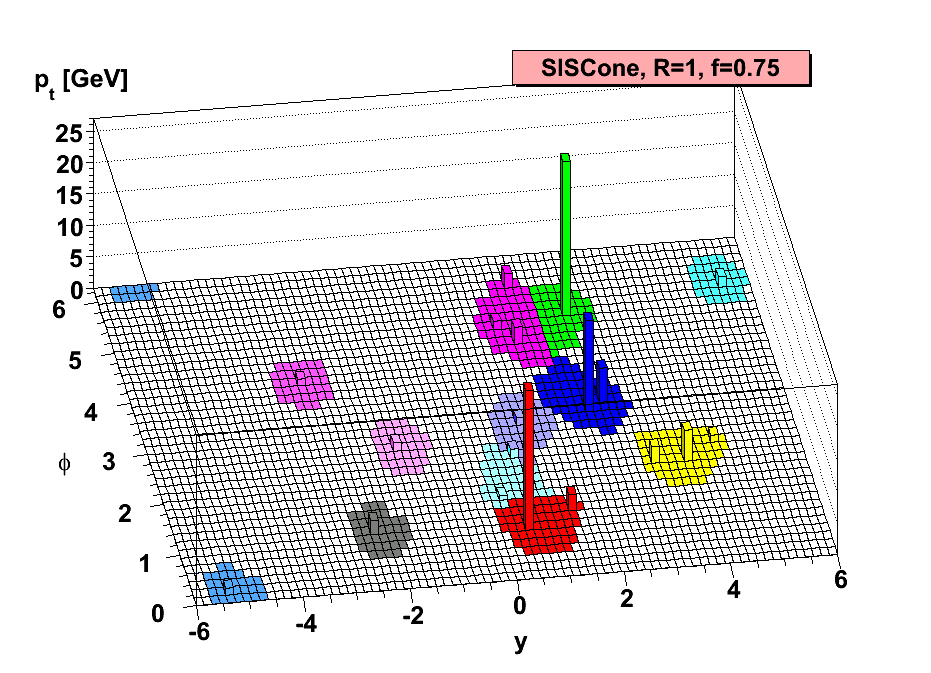
\includegraphics[width=\textwidth]{siscone.png}
            \caption[SISCONE]%
            {{\small SISCONE}}    
            \label{fig:mean and std of net34}
        \end{subfigure}
        \quad
        \begin{subfigure}[b]{0.475\textwidth}   
            \centering 
            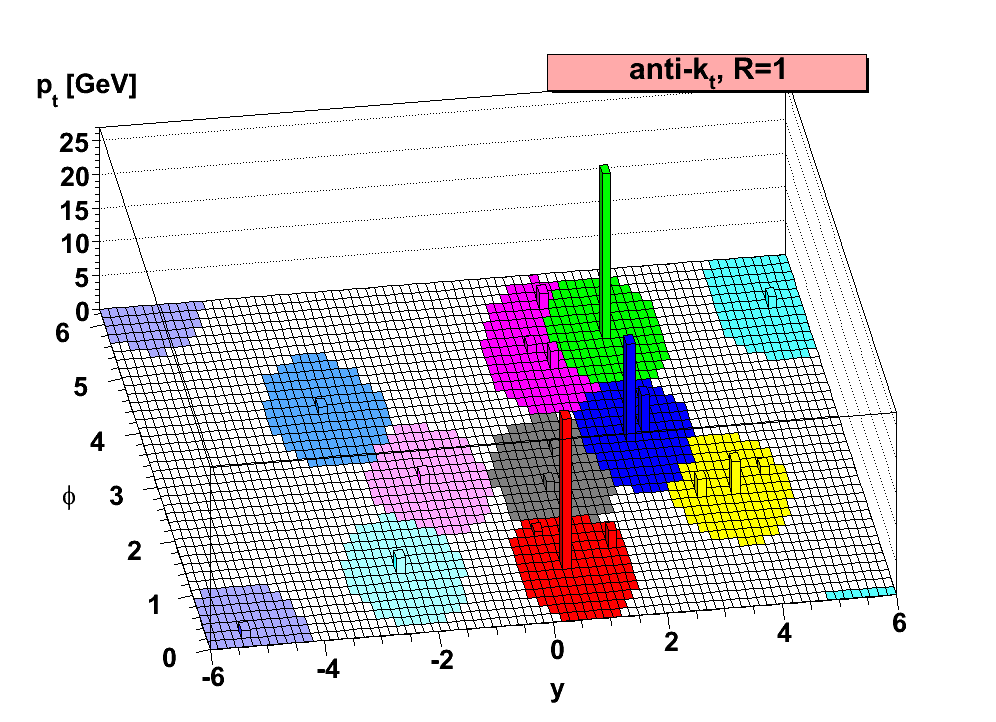
\includegraphics[width=\textwidth]{antikt.png}
            \caption[$anti k_T$]%
            {{\small $anti k_T$}}    
            \label{fig:mean and std of net44}
        \end{subfigure}
        \caption[ 4 farklı Jet algoritmasının parçacıkları sınıflandırması]
        {\small 4 farklı Jet algoritmasının parçacıkları sınıflandırması} 
        \label{fig:jetalgorithm}
    \end{figure}